\chapter{Usando \maggen}
\label{chap:usos}
\minitoc

Para usar \maggen\ debemos invocar la herramienta mediante la línea de comando, es decir, debemos contar con una terminal\footnote{En sistemas \textit{Windows} compatible: \textbf{Win+R} y luego \texttt{cmd} y en sistemas \textit{Unix}: \textbf{Alt+F2} y luego \texttt{xterm}} para su ejecución. Por cuestiones de simplicidad y flexibilidad de la herramienta, no se consideró el desarrollo de un \textit{front-end} para \maggen. Además, debemos tener en cuenta, que el usuario presentara interés en el resultado generado de \maggen\ y no de una innecesaria interfaz gráfica, que entorpecería su comportamiento combinatorio con otros comandos.
  
\maggen\ puede ser invocado utilizando una serie de parámetros que inciden directamente sobre el resultados producido por la herramienta. En el desarrollo de este capítulo trataremos estos temas en detalles y además analizaremos el uso del evaluador generado por \maggen. En la sección siguiente abordaremos detalles en la compilación e instalación de la herramienta.

\section{Compilación e Instalación de \maggen}
\maggen\ puede ser descargado desde el repositorio svn (\cite{svn-book}) utilizando el siguiente comando:
\begin{verbatim}
 svn checkout http://genevalmag.googlecode.com/svn/trunk/ maggen
\end{verbatim}

Una vez descargado \maggen\ contaremos con un directorio llamado {\sf maggen/}

Para compilar e instalar \maggen\ se deberán ejecutar en una terminal los siguientes comandos desde la carpeta {\sf /maggen} :
\begin{verbatim}
1.- maggen$ ./configure
2.- maggen$ make clean
3.- maggen$ make
4.- maggen$ sudo make install
\end{verbatim}

\subsection*{Directorio {\sf maggen}}
Luego de la compilación e instalación, el directorio raíz de \maggen\ se compone de lo siguiente:
\begin{itemize}
\item \textbf{/bin} Directorio que contiene módulos estáticos necesarios para la generación de código y uso del evaluador obtenido.
{\footnotesize \begin{verbatim}
 maggen$ ls -R bin/
 bin:
 lib

 bin/lib:
 Node.hpp  Plan.hpp
\end{verbatim} }
 
\item \textbf{/src} Directorio raíz en el que se encuentran todos los archivos fuentes.
{\footnotesize \begin{verbatim}
maggen$ ls -R src/ 
src/:
Attr_grammar  Builders  Expression_tree  maggen.cpp  Maglib.cpp  Parser  Util

src/Attr_grammar:
Attr_grammar.cpp  Attribute.cpp  Equation.cpp  Function.cpp  Rule.cpp  Sort.cpp  Symbol.cpp

src/Builders:
Builder_code.cpp  Builder_graphs.cpp  Builder_plans.cpp  Builder_visit_sequences.cpp

src/Expression_tree:
Expression.cpp  Expr_function.cpp  Expr_instance.cpp  Expr_leaf.cpp  Expr_literal.cpp  Expr_node.cpp

src/Parser:
Parser_AG.cpp  Semantics_actions.cpp  Semantics_checks.cpp

src/Util:
Utilities.cpp
\end{verbatim} }

\item \textbf{/include} Directorio raíz en el que se encuentran todos los archivos de cabecera.

{\footnotesize \begin{verbatim}
maggen$ ls -R include/
include/:
Attr_grammar  Builders  Expression_tree  Maglib.h  Parser  Util

include/Attr_grammar:
Attr_grammar.h  Attribute.h  Equation.h  Function.h  Rule.h  Sort.h  Symbol.h

include/Builders:
Builder_code.h  Builder_graphs.h  Builder_plans.h  Builder_visit_sequences.h

include/Expression_tree:
Expression.h  Expr_function.h  Expr_instance.h  Expr_leaf.h  Expr_literal.h  Expr_node.h

include/Parser:
Parser_AG.h  Semantics_actions.h  Semantics_checks.h

include/Util:
Utilities.h
\end{verbatim}}

\item \textbf{/scripts} Directorio que contiene scripts útiles para el usuario, por ejemplo: \texttt{dot2png.sh} para convertir a imagen \textit{png} los archivos de grafos y planes generados por \maggen.
{\footnotesize \begin{verbatim}
 maggen$ ls -R scripts/
 scripts/:
 dot2png.sh
\end{verbatim} }
 
\item \textbf{/examples} En este directorio se encuentran tres ejemplos de gramáticas para probar la herramienta.
{\footnotesize \begin{verbatim}
 maggen$ ls -R examples/
 examples/:
 ag_aritmetic  ag_count  ag_wuu_yang

 examples/ag_aritmetic:
 ag_aritmetic.cpp  ag_aritmetic.input

 examples/ag_count:
 ag_count.cpp  ag_count.input

 examples/ag_wuu_yang:
 ag_wuu_yang.cpp  ag_wuu_yang.input
\end{verbatim} }

\item \textbf{/doc} Directorio que contiene la documentación de la herramienta (doxygen).
\item \textbf{/Release} Directorio con los archivos compilados.
\item Archivos usados por \texttt{automake} y \texttt{autoconf} para generar los archivos \texttt{Makefile} y el script \texttt{configure} que permiten automatizar el proceso de compilación, empaquetado e instalación del proyecto.
\end{itemize}

Ahora ya estamos listos para empezar a usar \maggen, en las siguientes secciones analizaremos como usar la herramienta.

\section{Uso de \maggen: Parámetros y opciones}
\label{sec:uso-maggen}
La totalidad de parámetros y opciones de \maggen\ son opcionales. La sintaxis de invocación de la herramienta esta dada por:\\
\begin{center}\texttt{maggen [OPTIONS]}\end{center}
Las opciones son las siguientes:

\begin{description}
\item [-f  file] Definir el archivo de entrada de \maggen\ como \texttt{file}. Si omitimos esta opción \maggen\ espera la entrada por la entrada estándar (\texttt{cin}) hasta leer el carácter \texttt{EOF} (end of file)\footnote{En sistemas Unix el carácter \texttt{EOF} puede ser producido con \textbf{Ctrl+D} dentro de una consola de comandos.}.
\item [-i  header] Incluir \texttt{header} en la generación de código. Genera un \texttt{\#include ``header''} del archivo que referencia esa ruta. Dicha linea, \maggen\ la agrega al archivo generado.
\item [-fo folder] Define \texttt{folder} como el directorio de salida para \maggen. Si omitimos esta opción, \maggen\ usa el folder por defecto ``\textit{./out\_maggen/}''.
\item [-o  name] Define a \texttt{name} como el nombre de la clase y del archivo generado por \maggen. Si omitimos esta opción, \maggen\ usa por defecto el nombre ``\textbf{mag\_eval}''.
\item [-h] Muestra mensaje de ayuda.
\end{description}

A continuación observemos algunos ejemplo de invocación de \maggen.
\begin{itemize}
\item Si invocamos:\\ \texttt{./maggen -h} obtenemos el siguiente mensaje de ayuda:

\begin{figure}[!ht]\centering
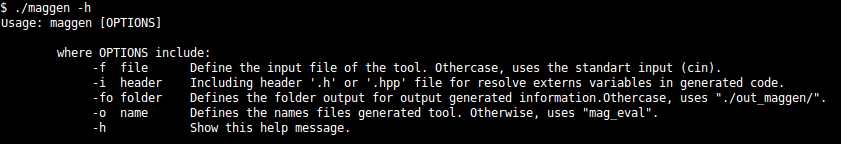
\includegraphics[width=350pt,height=60pt]{help.png}
\caption{\label{fig:outhelp} Información de ayuda de \maggen.}
\end{figure}

\item Si invocamos: \\ \texttt{./maggen -fo ./Out\_wuu\_yang -o evalmag -f ./examples/ag\_wuu\_yang/ag\_wuu\_yang.input}. \\ Especificamos como archivo de entrada a \texttt{ag\_wuu\_yang.input}, como directorio de salida \texttt{./Out\_wuu\_yang} y el nombre de la clase (y archivo) generada con el nombre \texttt{evalmag}. La figura \ref{fig:outnormal} muestra la salida de esta invocación.

\begin{figure}[!ht]\centering
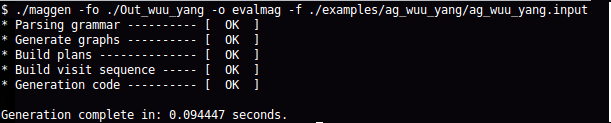
\includegraphics[width=350pt,height=70pt]{normal.png}
\caption{\label{fig:outnormal} Usando \maggen\ con opciones.}
\end{figure}

\item Si invocamos a \maggen\ sin la opción \texttt{-f} (independientemente que usemos o no las demás opciones) se espera la entrada por entrada estándar. Esto nos permite poder utilizar a \maggen\ en conjunto con otros comandos, Ejemplo:\\ \texttt{cat file | maggen -fo ./out/}.\\ Esto muestra a \maggen\ en conjunto con \texttt{cat} usando una tubería (\texttt{pipe} o \texttt{|}).

\end{itemize}

La salida de \maggen\ esta ordenada a través de directorio bien definidos que marcan el proceso de funcionamiento de la herramienta en casa etapa. A continuación analizaremos la salida de \maggen\ para la invocación:\\

\small\texttt{./maggen -fo ./Out\_wuu\_yang -o maggen -f ./examples/ag\_wuu\_yang/ag\_wuu\_yang.input}.\\

La totalidad de la información generada por la herramienta es mostrada en la figura \ref{fig:outmaggen}.

\begin{figure}[!ht]\centering
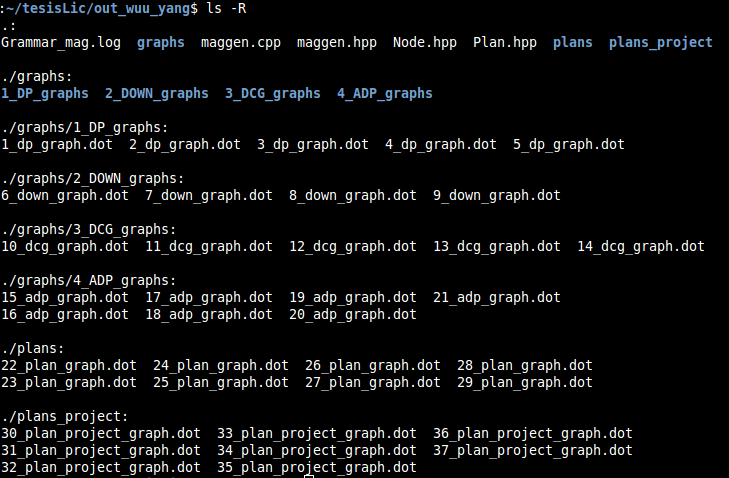
\includegraphics[width=350pt,height=229pt]{out_all.png}
\caption{\label{fig:outmaggen} Salida de \maggen: Directorios y archivos.}
\end{figure}

Dicha información es almacenada en la ruta \texttt{./Out\_wuu\_yang}, dentro de la cual podemos observar:

\begin{description}
\item [Archivos maggen.cpp y maggen.cpp] Código C++ del evaluador estático. Es la \textbf{salida principal de} \maggen.

\item [Archivos Plan.hpp y Node.hpp] Código C++ con definiciones y declaraciones necesarias para la ejecución de ``maggen''.

\item [Archivo ``Grammar\_mag.log''] Este contiene la gramática parseada. Se debe tener en cuenta el análisis de este archivo, esto permite encontrar posibles errores en la interpretación del archivo de entrada a \maggen. Tal como se muestra la gramática en este archivo, es la que la herramienta a utilizado para la generación del evaluador.

\item [Directorio ``graphs''] Contiene los 4 tipos de grafos construidos por \maggen\ en el proceso visto en la sección \ref{subsec:graph}. Los mismos están ordenados por 4 directorios diferentes denominados: \textit{1\_DP\_graphs}, \textit{2\_DOWN\_graphs}, \textit{3\_DCG\_graphs}, \textit{4\_ADP\_graphs}. Cada unos de ellos contiene archivos \texttt{.dot} para cada grafo creado. Este directorio, además, es utilizado para el caso que se detecte planes cíclicos, donde se almacenan los grafos que producen dependencias cíclicas en un solo directorio y se omiten los demás grafos.

\item [Directorio ``plans''] Contiene archivos \texttt{.dot} con los planes generados por \maggen.

\item [Directorio ``plans project''] Contiene archivos \texttt{.dot} con los planes proyectados generados por \maggen.
\end{description}

\section{Uso del evaluador generado}

Para el usos del evaluador generado por \maggen\ necesitamos los 4 archivos generados en el directorio de salida, siguiendo con la salida de la sección anterior, ellos son:
\begin{itemize}
\item maggen.hpp.
\item maggen.cpp.
\item Plan.hpp.
\item Node.hpp.
\end{itemize}

El evaluador generado por \maggen\ puede ser usado como un modulo C++ en conjunto con otro proyecto. En esta sección seguiremos con un ejemplo el uso del evaluador para el ejemplo Wuu Yang, el cual se ha tratado en los capítulos anteriores (Ver entrada a \maggen\ en el apéndice \ref{append:agwuuyang}).

Como bien hemos visto en secciones anteriores, la entrada del evaluador generado por \maggen\ es un AST. El siguiente módulo de código C++ describe un AST para la gramática del ejemplo de Wuu Yang.

\lstinputlisting[basicstyle=\tiny, language=c++, numbers=left]{input_file_code/ag_wuu_yang.cpp}

Observemos el AST con el siguiente diagrama:

\begin{center}
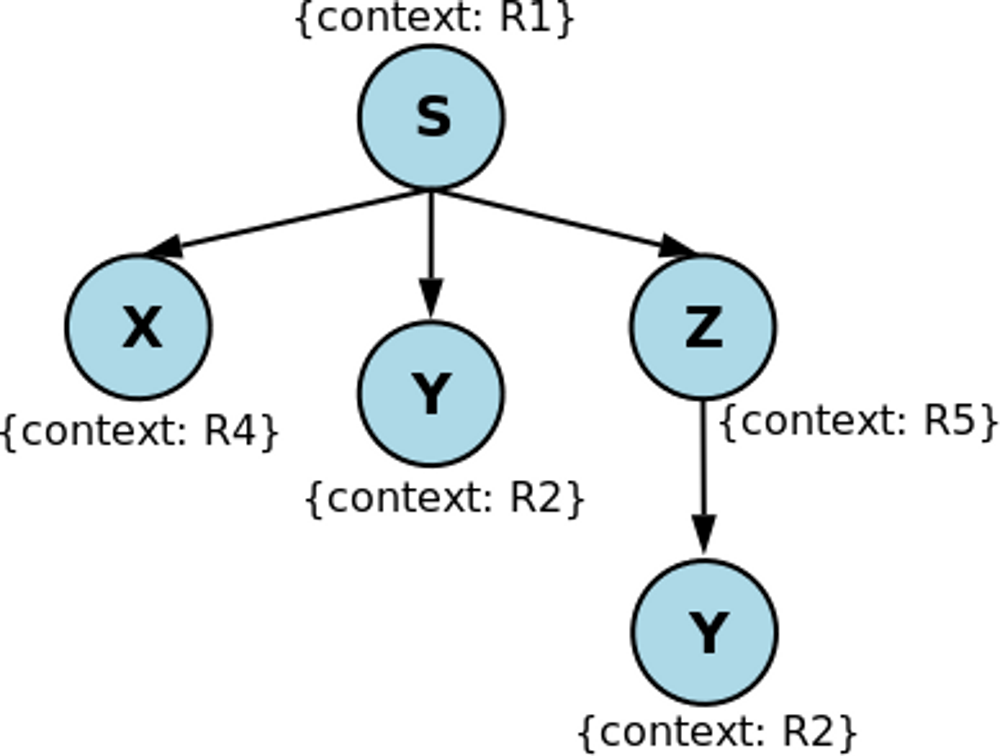
\includegraphics[width=200pt,height=154pt]{ast.png}
\end{center}

Los atributos de cada símbolo del AST esta con valores indefinidos, veamos en la siguiente imagen con la compilación e invocación del evaluador generado por \maggen\ para computar los atributos de los símbolos del AST.

\begin{center}
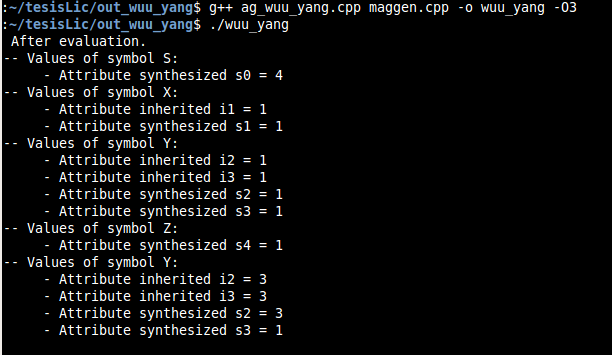
\includegraphics[width=350pt,height=203pt]{ast-computed.png}
\end{center} 

Analicemos los valores de los atributos de cada símbolo en la siguiente tabla:

\begin{center}\begin{tabular}{|| c | c | l ||}
\hline \hline

\rowcolor{gris} \textbf{Símbolo}&\textbf{Atributo}&\textbf{Evaluación}\\ \hline

\multirow{2}{*}{\textbf{S}} & \multirow{2}{*}{s0} & \texttt{(eq 1) S.s0 = X.s1 + Y.s2 + Y.s3 + Z.s4} \\ 
                           &                     & \textbf{S.s0 = 4} \\ \hline

\multirow{4}{*}{\textbf{X}} & \multirow{2}{*}{i1} & \texttt{(eq 2) X.i1 = Y.s3} \\ 
                           &                     & \textbf{X.i1 = 1.} \\ \cline{2-3}
                           & \multirow{2}{*}{s1} & \texttt{(eq 9) X.s1 = X.i1} \\ 
                           &                     & \textbf{X.s1 = 1.} \\ \hline

\multirow{7}{*}{\textbf{Y}} &                 s3  & \texttt{(eq 6)} \textbf{Y.s3 = 1} \\ \cline{2-3}
                           & \multirow{2}{*}{s2} &    \texttt{(eq 5) Y.s2 = Y.i2} \\
                           &                     & \textbf{Y.s2 = 1} \\ \cline{2-3}
                           & \multirow{2}{*}{i2} & \texttt{(eq 3) Y.i2 = X.s1} \\
                           &                     & \textbf{Y.i2 = 1} \\ \cline{2-3}
                           & \multirow{2}{*}{i3} & \texttt{(eq 4) Y.i3 = Y.s2} \\
                           &                     & \textbf{Y.i3 = 1} \\ \hline

\multirow{2}{*}{\textbf{Z}} & \multirow{2}{*}{S4} & \texttt{(eq 10) Z.s4 = Y.s3} \\
                           &                     & \textbf{Z.s4 = 1} \\ \hline

\multirow{7}{*}{\textbf{Y}} &                  s3 & \texttt{(eq 6)} \textbf{Y.s3 = 1} \\ \cline{2-3}
                           & \multirow{2}{*}{s2} &    \texttt{(eq 5) Y.s2 = Y.i2} \\
                           &                     & \textbf{Y.s2 = 3} \\ \cline{2-3}
                           & \multirow{2}{*}{i2} & \texttt{(eq 3) Y.i2 = X.s1} \\
                           &                     & \textbf{Y.i2 = 3} \\ \cline{2-3}
                           & \multirow{2}{*}{i3} & \texttt{(eq 4) Y.i3 = Y.s2} \\
                           &                     & \textbf{Y.i3 = 3} \\
\hline \hline
\end{tabular}\end{center}

Tal como analizamos en el ejemplo anterior, el evaluador generado por \maggen\ podría ser utilizado con todos lo AST posibles. Esto es, debido a que el evaluador contiene las secuencias de visita previamente computadas para hacer la tarea de evaluación con una notoria ganancia de tiempo. Entonces podríamos invocar al evaluador, además, con los demás AST que se desprenden con la gramática del ejemplo de Wuu Yang. En la figura \ref{fig:allast} podemos ver la totalidad de AST.

\begin{figure}[!ht]\centering
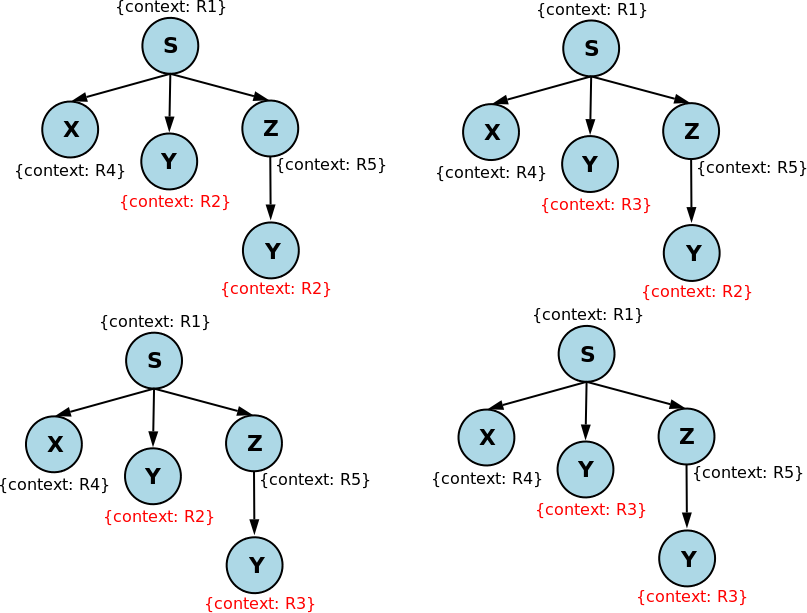
\includegraphics[width=350pt,height=266pt]{ast-all.png}
\caption{\label{fig:allast} AST para ejemplo de Wuu Yang.}
\end{figure}

Notar que el ejemplo Wuu yang analizado es considerablemente simple, pero podemos encontrar gramáticas muy simples en la cual los posibles AST sea una cantidad considerable, es en este punto donde el evaluador generado por \maggen\ adquiere mayor potencial y utilidad.

\section{Mensajes y avisos}

En los cuadros \ref{table:mensajes-err} y \ref{table:mensajes-av} analizamos la descripción de los posibles errores y avisos que se deben tener en cuenta cuando usamos \maggen.
% \newpage
{
\begin{small}
\begin{longtable}{| p{5cm} || p{5cm} | p{5cm} |}

\hline

\rowcolor{gris} \textbf{Mensaje} & \textbf{Descripción} & \textbf{Ayuda} \\ \hline \hline

ERROR: operator non-associtive using wrong use: \textit{OP} & El operador \textit{OP} es non\_assoc y se pretende una asociación del mismo, en alguna expresión. & Modifique la definición del operador o chequee la expresión.\\ \hline

ERROR: Symbol Non-Teminal \textit{SYMB} uses in the right part without rule & El símbolo \textit{SYMB}, usado en la gramática, no tiene regla que lo defina. & Chequee los símbolos usados o defina una regla para el símbolo \textit{SYMB}. \\ \hline

ERROR: \textit{SYMB} [\textit{NUM}]. \textit{ATTR} type synthetized, haven't an equation that defines it. & Gramática mal definida, atributo sintetizado \textit{ATTR} sin ecuación que lo defina. Para mas información chequee la sección \ref{subsec:check} & Defina ecuación para la instancia o chequee la definición de la gramática. \\ \hline

ERROR: \textit{SYMB} [\textit{NUM}].\textit{ATTR} type inherited, haven't an equation that defines it. & Gramática mal definida, atributo heredado \textit{ATTR} sin ecuación que lo defina. Para mas información chequee la sección \ref{subsec:check} & Defina ecuación para la instancia o chequee la definición de la gramática. \\ \hline

ERROR: \textit{SYMB} [\textit{NUM}].\textit{ATTR} type synthetized, is defined outside his scope. & La instancia \textit{SYMB} [\textit{NUM}].\textit{ATTR} esta definida fuera de su regla de alcance. & Defina ecuación en el alcance de la regla o chequee la instancia usada. \\ \hline

ERROR: the file input non-exist & El archivo de entrada a \maggen\ no existe o es inaccesible. & Chequee la ruta del archivo de entrada. \\ \hline

ERROR: Parsing Failed, the following text will not be able to parse: \ldots & Error sintáctico en la definición de la gramática. Para mas información chequee la sección \ref{sec:lenguajeMAG} & Revise la sintaxis del lenguaje de definición para \maggen\ y modifique su definición. \\ \hline

ERROR: non-terminal symbol \textit{SYMB} used does not belong to the rule: \textit{R} & Instancia utilizada fuera de su entorno. Símbolo de la instancia no pertenece al entorno de la regla. & Revise el uso de la instancia o modifique la regla \textit{R}.  \\ \hline

ERROR: Index \textit{NUM} of symbol  \textit{SYMB} incorrect. & Índice \textit{NUM} de instancia fuera de rango. No corresponde el índice con el orden sintáctico del símbolo en la regla. & Revise el índice \textit{NUM} o modifique la definición de la regla.  \\ \hline 

ERROR: \textit{ATTR} Attribute non-existent. Check the attributes used in the symbols. & El atributo no pertenece al símbolo. & Defina el atributo \textit{ATTR} o modifique el uso de esa instancia. \\ \hline

ERROR: Type not expected from l\_value." & Error de tipo. El tipo que sintetiza la expresión r\_value no corresponde con el tipo de l\_value & Revise la expresión en busca de mal uso de operadores, o modifique los tipos de los atributos u operadores. \\ \hline
 
ERROR: infix operator non-exist: \textit{OP-IN}. & El operador infijo \textit{OP-IN} utilizado en la expresión no esta definido o esta siendo usado con tipos erróneos. & Defina el operador o modifique la expresión. \\ \hline
 
ERROR: Function non-exist: \textit{F}. & La función \textit{F} utilizada en la expresión no esta definida o esta usada con tipos erróneos. & Defina la función o modifique la expresión. \\ \hline
 
ERROR: postfix operator non-exist: \textit{OP-POS}. & El operador posfijo \textit{OP-POS} utilizado en la expresión no esta definido o esta usado con tipos erróneos. & Defina el operador o modifique la expresión. \\ \hline 

ERROR: prefix operator non-exist: \textit{OP-PRE}. & El operador prefijo \textit{OP-PRE} utilizado en la expresión no esta definido o esta usado con tipos erróneos. & Defina el operador o modifique la expresión. \\ \hline 

ERROR: The grammar isn't extended grammar. & Error en la definición de la gramática, la misma no cumple con la propiedad de gramática extendida. Ver detalles en sección \ref{sec:def-CFG} & Chequee la definición de la gramática para que cumpla la propiedad.(sección grammar extended) \\ \hline

ERROR: the path \textit{PATH} is invalid or inaccessible. & El camino (PATH) es inexistente o inaccesible. & Verifique la ruta e invoque a \maggen\ nuevamente. \\ \hline

ERROR: One o more graph ADP has an cycle in its dependencies. Look the folder \textit{PATH-OUTPUT}. & El proceso de \maggen\ tuvo que ser abortado, debido a la existencia de planes con dependencias circulares. & Chequee la definición de las ecuaciones que se vinculan con los grafos mostrados en \textit{PATH-OUTPUT}. \\ \hline 

ERROR: Path non exist: \textit{PATH}. & Ruta errónea o inaccesible. & Modifique la ruta PATH o ingrese una nueva. \\ \hline 

ERROR: maggen wrong uses. & Mal uso de \maggen, uno de los argumentos es erróneo, en la invocación. & Modifique los argumentos. Para mas detalle chequee sección \ref{sec:uso-maggen} \\ \hline

ERROR: Index out bounds: combined ADP graphs.& Error fatal en la generación de contextos para la construcción de ADP. & Chequee la entrada a \maggen.\\ 
\hline \hline
\caption{Tabla con mensajes de error en \maggen.}\label{table:mensajes-err}
\end{longtable}
\begin{longtable}{| p{5cm} || p{5cm} | p{5cm} |}

\hline

\rowcolor{gris} \textbf{Mensaje} & \textbf{Descripción} & \textbf{Ayuda} \\ \hline \hline

WARNING: Symbol Non-Teminal  \textit{SYMB} unreachable. & El símbolo \textit{SYMB} es inalcanzable desde la regla inicial de la gramática. El mismo es ignorado en el proceso de computo. & Chequee la gramática de entrada a \maggen\ o elimine el símbolo en caso de uso innecesario. \\ \hline

WARNING: Sort duplicate was ignored: $-->$ \textit{S} & La declaración del sort \textit{S} esta duplicada. \maggen\ ignora dicha linea. & Elimine la declaración del sort \textit{S} o modifique la misma en caso de declaración de sort distinto. \\ \hline

WARNING: Declaration duplicate was ignored: $-->$ \textit{F} & La declaración de la función \textit{F} esta duplicada. \maggen\ ignora dicha línea. & Elimine la declaración de la función \textit{F} o modifique la misma en caso de declaración de función distinta. \\ \hline

WARNING: Ignores the eq \textit{E} duplicate definition for \textit{IN} in rule: $-->$ \textit{R} & La ecuación \textit{E} para la instancia \textit{IN} en la regla \textit{R} es ignorada por \maggen, debido a que la instancia \textit{IN} ya tiene ecuación que la defina. & Chequee las ecuaciones que definen la instancia \textit{IN} y elimine una o verifique posibles errores en la ecuación. \\ \hline
\caption{Tabla con mensajes de avisos en \maggen.}\label{table:mensajes-av}
\end{longtable}
\end{small}}
\normalsize

En los cuadros anteriores se pudo analizar los errores y los avisos en el uso de \maggen. Esta diferencia en los mensajes, se hace en el sentido de que, los avisos, no son considerados errores fatales en el proceso de la herramienta y por ende no es necesario abortar el funcionamiento. Los errores considerados avisos, \textbf{son ignorados} dentro del funcionamiento interno de \maggen.

Al igual como analizamos para \maggen, a continuación veamos los mensajes de error en el uso del evaluador generado:

\begin{table}[h]
\begin{small}
\begin{tabular}{| p{5cm} || p{5cm} | p{5cm} |}

\hline \hline

\rowcolor{gris} \textbf{Mensaje} & \textbf{Descripción} & \textbf{Ayuda} \\ \hline

ERROR: the AST input is wrong create. Context rule does not exist. & Los nodos del AST describen una combinación de reglas no posible en la gramática de entrada. & Revise el AST o modifique la gramática y genere nuevamente el evaluador con \maggen. \\ \hline

ERROR: the AST input is wrong create. Evaluation plan does not exist. & El orden de evaluación impuesto al nodo no corresponde. & Revise si la gramática esta bien especificada. \\ \hline

ERROR: Fatal action. & Se desea invocar a la computación de una ecuación errónea e inexistente. & Chequee el AST de entrada al evaluador. \\ \hline
\end{tabular}
\caption{Mensajes de error del evaluador generado por \maggen.}
\end{small}
\end{table}

El error más importante y común cuando se usa el evaluador generado por \maggen\ esta dado por el AST de entrada. Es aconsejable que se chequee de manera exhaustiva la creación de estos AST para evitar complicaciones.
